\documentclass[nooutcomes]{ximera}
%% handout
%% space
%% newpage
%% numbers
%% nooutcomes

%I added the commands here so that I would't have to keep looking them up
%\newcommand{\RR}{\mathbb R}
%\renewcommand{\d}{\,d}
%\newcommand{\dd}[2][]{\frac{d #1}{d #2}}
%\renewcommand{\l}{\ell}
%\newcommand{\ddx}{\frac{d}{dx}}
%\everymath{\displaystyle}
%\newcommand{\dfn}{\textbf}
%\newcommand{\eval}[1]{\bigg[ #1 \bigg]}

%\begin{image}
%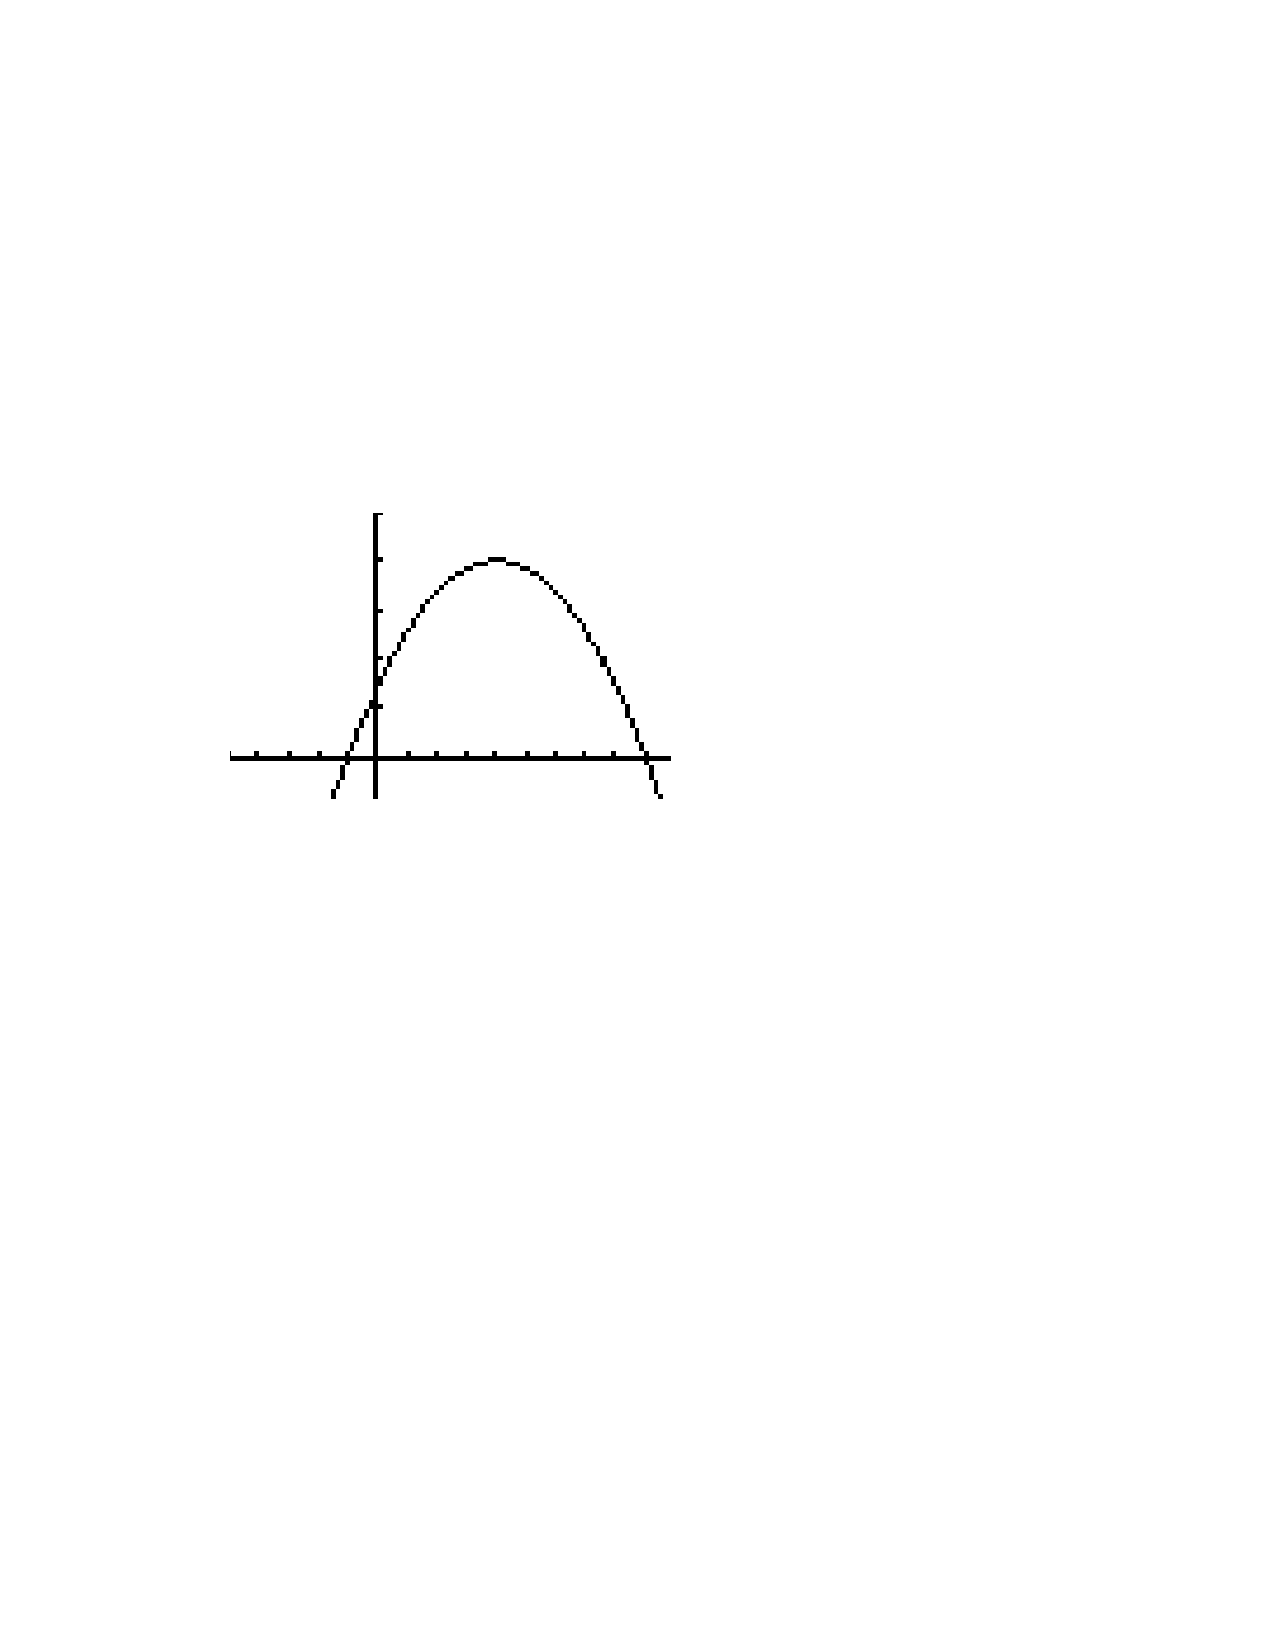
\includegraphics[trim= 170 420 250 180]{Figure1.pdf}
%\end{image}


\newcommand{\RR}{\mathbb R}
\renewcommand{\d}{\,d}
\newcommand{\dd}[2][]{\frac{d #1}{d #2}}
\renewcommand{\l}{\ell}
\newcommand{\ddx}{\frac{d}{dx}}
\newcommand{\dfn}{\textbf}
\newcommand{\eval}[1]{\bigg[ #1 \bigg]}

\usepackage{multicol}

\renewenvironment{freeResponse}{
\ifhandout\setbox0\vbox\bgroup\else
\begin{trivlist}\item[\hskip \labelsep\bfseries Solution:\hspace{2ex}]
\fi}
{\ifhandout\egroup\else
\end{trivlist}
\fi} %% we can turn off input when making a master document

\title{Recitation \#16 - 4.2 What Derivatives Tell Us (Solutions)}  

\begin{document}
\begin{abstract}		\end{abstract}
\maketitle

\section*{Warm up:} 
Fill in the following blanks with the correct choice of the words from this list:
$$ \text{Increasing, decreasing, positive, negative, concave up, concave down} $$

	\begin{enumerate}
	
	%part a
	\item  If you know $f''(x) > 0$, then you know $f'(x)$ is \underline{\hspace{3cm}} and $f(x)$ is \underline{\hspace{3cm}}.
		\begin{freeResponse}
		increasing, concave up
		\end{freeResponse}
		
			
				
	%part b
	\item  If you know $g'(x) < 0$ and decreasing, then you know $g(x)$ is \underline{\hspace{3cm}} and \underline{\hspace{3cm}}.
		\begin{freeResponse}
		decreasing, concave down
		\end{freeResponse}
		
			
				
	%part c
	\item  If you know $h(x)$ is positive, increasing, and concave down, then you know $h'(x)$ is \underline{\hspace{3cm}} and \underline{\hspace{3cm}} and that $h''(x)$ is \underline{\hspace{3cm}}.
		\begin{freeResponse}
		positive, decreasing, negative
		\end{freeResponse}
		
			
				
	\end{enumerate}	
		
		
		

	
	
	
	
	

\section*{Group work:}



%problem 1
\begin{problem}
Let $f(x) = \frac{1}{1 + x^2}$ on the interval $[-2,2]$.  Find the following for $f$:

	\begin{enumerate}
	
	\item  $f'$ and $f''$
	
		\begin{freeResponse}
			\begin{align*}
			f'(x) &= \frac{(1+x^2)(0) - 1(2x)}{(1+x^2)^2} \\
			&= \frac{-2x}{(1+x^2)^2}
			\end{align*}
			
			\begin{align*}
			f''(x) &= \frac{(1+x^2)^2(-2) - (-2x)(2)(1+x^2)(2x)}{(1+x^2)^4} \\
			&= \frac{-2(1+x^2) + 8x^2}{(1+x^2)^3} \\
			&= \frac{6x^2 - 2}{(1+x^2)^3}
			\end{align*}
		\end{freeResponse}
		
	\item  Critical points
	
		\begin{freeResponse}
		Since $1+x^2 > 0$ for all $x$, $f$ is differentiable over all real numbers.  Thus all critical points of $f$ occur when $f'(x) = 0$ and $x \in (-2,2)$.  But a fraction equals 0 if and only if its numerator equals 0.  So
		$$ f'(x) = 0 \qquad \Longrightarrow \qquad -2x = 0 \qquad \Longrightarrow \qquad x=0 $$
		Hence, the only critical point is $x=0$.  
		\end{freeResponse}
		
	\item  Intervals where $f$ is increasing and decreasing
	
		\begin{freeResponse}
		Because $f'$ doesn’t change sign in the interval $(-2,0)$, we can use a test point in this interval to determine the sign of $f'$ on the interval.  Let us chose $x=-1$ and, similarly on $(0,2)$, choose $x=1$.
		$$ f'(-1) = \frac{2}{4} > 0 $$
		$$ f'(1) = \frac{-2}{4} < 0 $$
		So we have the following picture:
		
%%%%%%%%%%%%%%%%%%%%%%%%%%%%%%%%%%%%%%%%%%%%%%%%%%%%%%%%%%%%%%%%%%%%%%%%%%%%%%%%%%%%%%
		
\begin{center}
\begin{image}
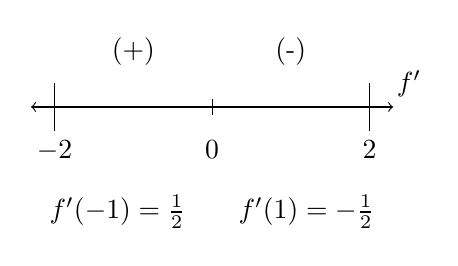
\begin{tikzpicture}

%\draw[help lines] (-2,-2) grid (2,2);

\draw [<->] (-2.3,0) -- (2.3,0);
\draw (-2,0.3) -- (-2,-0.3);
\draw (0,0.1) -- (0,-0.1);
\draw (2,0.3) -- (2,-0.3);

\draw (-2,-0.3)node[below]{$-2$};
\draw (0,-0.3)node[below]{$0$};
\draw (2,-0.3)node[below]{$2$};
\draw (-1.2,-1)node[below]{$f'(-1) = \frac{1}{2}$};
\draw (1.2,-1)node[below]{$f'(1) = - \frac{1}{2}$};
\draw (-1,1)node[below]{(+)};
\draw (1,1)node[below]{(-)};
\draw (2.5,0)node[above]{$f'$};


\end{tikzpicture}
\end{image}
\end{center}

%%%%%%%%%%%%%%%%%%%%%%%%%%%%%%%%%%%%%%%%%%%%%%%%%%%%%%%%%%%%%%%%%%%%%%%%%%%%%%%%%%%%%%%%

		Thus, $f'$ is positive on the interval $(-2,0)$ and negative on $(0,2)$, and therefore $f$ is increasing on $(-2,0)$ and decreasing on $(0,2)$.  
		\end{freeResponse}
		
	\item  Local extrema (and check your answers with both the first and second derivative tests)
	
		\begin{freeResponse}
		At $x=0$, $f'$ changes sign from positive to negative.  Thus $f$ goes from increasing to decreasing, and therefore by the first derivative test $x=0$ is a local maximum of $f$.  
		
		For the second derivative test, we have that
		$$ f''(0) = \frac{6(0)^2 - 2}{(1+0^2)^3} = \frac{-2}{1} = -2 < 0 $$
		and thus we again conclude that $x=0$ is a local maximum of $f$.
		\end{freeResponse}
		
	\item  Intervals of concavity
	
		\begin{freeResponse}
		To find points were $f''$ may change signs, we need to find where $f''(x)=0$ or $f''(x)$ does not exist.  $f''(x)$ exists everywhere in our domain so we are only looking for where $f''(x)=0$.  So we solve
		\begin{align*}
  		& \frac{6{{x}^{2}}-2}{{{(1+{{x}^{2}})}^{3}}}=0 \\ 
 		& 6{{x}^{2}}-2=0 \\ 
 		& {{x}^{2}}=\frac{2}{6} \\ 
 		& x=\pm \frac{1}{\sqrt{3}} \\ 
		\end{align*}
		Picking test points of $-1, 0, $ and $1$, we have that
		\begin{align*}
		& f''(-1) = \frac{6-2}{2^3} = \frac{4}{8} > 0 \\
		& f''(0) = \frac{0-2}{1^3} = \frac{-2}{1} < 0 \\
		& f''(1) = \frac{6-2}{2^3} = \frac{4}{8} > 0 \\
		\end{align*}
		So we have the following picture:
		
%%%%%%%%%%%%%%%%%%%%%%%%%%%%%%%%%%%%%%%%%%%%%%%%%%%%%%%%%%%%%%%%%%%%%%%%%%%%%%%%%%%%%%
		
\begin{center}
\begin{image}
\begin{tikzpicture}

%\draw[help lines] (-2,-2) grid (2,2);

\draw [<->] (-4.6,0) -- (4.6,0);
\draw (-4,0.3) -- (-4,-0.3);
\draw (-1.1547,0.1) -- (-1.1547,-0.1);
\draw (1.1547,0.1) -- (1.1547,-0.1);
\draw (4,0.3) -- (4,-0.3);

\draw (-4,-0.3)node[below]{$-2$};
\draw (-1.1547,-0.3)node[below]{$- \frac{1}{\sqrt{3}}$};
\draw (1.1547,-0.3)node[below]{$\frac{1}{\sqrt{3}}$};
\draw (4,-0.3)node[below]{$2$};
\draw (-3,-2)node[below]{$f''(-1) = \frac{1}{2}$};
\draw (0,-2.2)node[below]{$f''(0) = -2$};
\draw (3,-2)node[below]{$f''(1) = \frac{1}{2}$};
\draw (-2.5,1)node[below]{(+)};
\draw (0,1)node[below]{(-)};
\draw (2.5,1)node[below]{(+)};
\draw (5,0)node[above]{$f''$};


\end{tikzpicture}
\end{image}
\end{center}

%%%%%%%%%%%%%%%%%%%%%%%%%%%%%%%%%%%%%%%%%%%%%%%%%%%%%%%%%%%%%%%%%%%%%%%%%%%%%%%%%%%%%%%%

		
		
		Thus, $f$ is concave down on $\left( - \frac{1}{\sqrt{3}}, \frac{1}{\sqrt{3}} \right)$ and concave up on \\ 
		$\left( -2, - \frac{1}{\sqrt{3}} \right) \cup \left( \frac{1}{\sqrt{3}}, 2 \right)$
		\end{freeResponse}
		
	\item  Inflection points
	
		\begin{freeResponse}
		To find the inflection points, we need to find where $f''(x)=0$ or $f''(x)$ does not exist, \dfn{and} where$f''$changes sign.  We found these values in part (e):
		\begin{align*}
 		 & f\left( \frac{1}{\sqrt{3}} \right)=\frac{3}{4} \\ 
 		& f\left( -\frac{1}{\sqrt{3}} \right)=\frac{3}{4} \\ 
		\end{align*}  
		So our inflection points are: $\left( -\frac{1}{\sqrt{3}},\frac{3}{4} \right),\left( \frac{1}{\sqrt{3}},\frac{3}{4} \right)$
		\end{freeResponse}
		
	\item  Absolute extrema
	
		\begin{freeResponse}
		We need to check the critical points of $f$ and the endpoints of the interval:
		\begin{align*}
  		& f(-2)=\frac{1}{5} \\ 
 		& f(0)=1 \\ 
 		& f(2)=\frac{1}{5} \\ 
		\end{align*}
		So the absolute maximum value of $f$ on $[-2,2]$ is $f(0)=1$.  Both $f(-2)=\frac{1}{5}$ and $f(2)=\frac{1}{5}$ are the absolute minimum values of $f$ on $[-2,2]$.
		
		The graph of the function looks like:
		
%%%%%%%%%%%%%%%%%%%%%%%%%%%%%%%%%%%%%%%%%%%%%%%%%%%%%%%%%%%%%%%%%%%%%%%%%%%%%%%%%%%%%%%%
\begin{center}
\begin{image}
\begin{tikzpicture}[xscale=2,yscale=2]

\draw [<->] (0,2) -- (0,0) -- (3,0);
\draw [<->] (0,-1) -- (0,0) -- (-3,0);
\draw[red, ultra thick, domain=-2:2] plot (\x, {1/(1+(\x)^2)});
\draw (-2,0.1) -- (-2,-0.1);
\draw (2,0.1) -- (2,-0.1);
\draw (-2,-0.3)node[below]{$-2$};
\draw (2,-0.3)node[below]{$2$};
\draw (-0.57735,0.1) -- (-0.57735,-0.1);
\draw (0.57735,0.1) -- (0.57735,-0.1);
\draw (-0.57735,-0.2)node[below]{$- \frac{1}{\sqrt{3}}$};
\draw (0.57735,-0.2)node[below]{$\frac{1}{\sqrt{3}}$};

\end{tikzpicture}
\end{image}
\end{center}
%%%%%%%%%%%%%%%%%%%%%%%%%%%%%%%%%%%%%%%%%%%%%%%%%%%%%%%%%%%%%%%%%%%%%%%%%%%%%%%%%%%%%%%%


		\end{freeResponse}
	
	\end{enumerate}
		
\end{problem}







	
	
	
	
	
	
	
	
	

	










								
				
				
	














\end{document} 


















